% Asset ID: A21ParametricEquationsTikZ-003
% Source: Transcript section 2; CCEA A21-CG-LO001.
% Related lesson section: Worked Example 3.
% Purpose: Show the circle from x=sin t+2, y=cos t-3.

\documentclass[tikz,border=8pt]{standalone}
\usepackage{amsmath}
\usepackage{pgfplots}
\pgfplotsset{compat=1.18}
\begin{document}
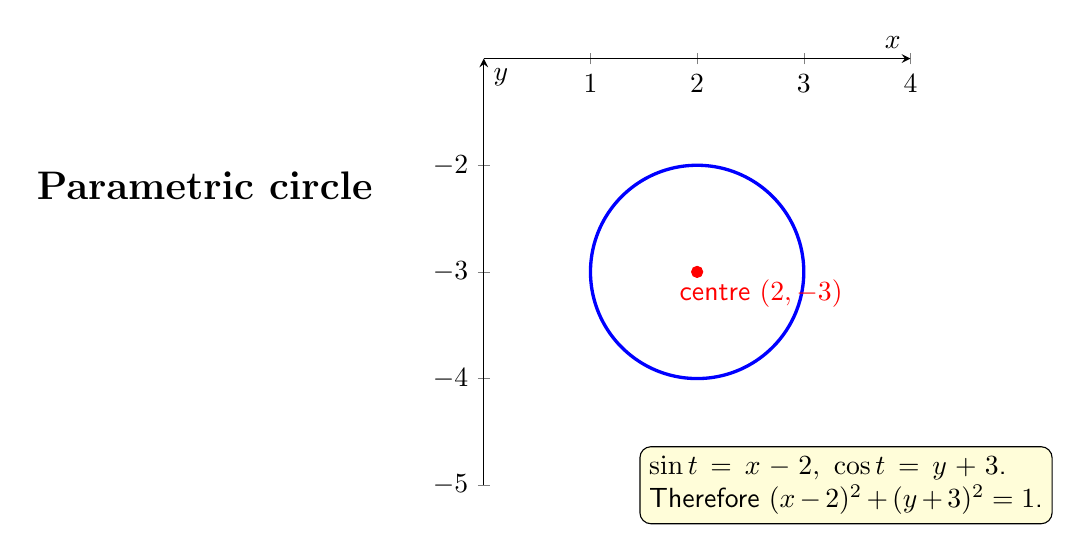
\begin{tikzpicture}[font=\sffamily]

\node[anchor=west, font=\bfseries\Large] at (-5.8,3.8) {Parametric circle};
\begin{axis}[width=8cm,height=7cm,axis lines=middle,xmin=0,xmax=4,ymin=-5,ymax=-1,axis equal image,xlabel={$x$},ylabel={$y$}]
\addplot[domain=0:360,samples=200,blue,very thick] ({2+sin(x)},{-3+cos(x)});
\addplot[only marks,red] coordinates {(2,-3)};
\node[red] at (axis cs:2.6,-3.2) {centre \((2,-3)\)};
\end{axis}
\node[draw, rounded corners, fill=yellow!15, text width=5cm] at (4.6,0) {\(\sin t=x-2,\ \cos t=y+3\). Therefore \((x-2)^2+(y+3)^2=1\).};

\end{tikzpicture}
\end{document}
